\paragraph{Classification with non-linear decision boundaries}
Rather than fitting a support vector classifier using $p$ features
we could instead fit a support vector classifier using $2p$ features,
then we get for $\left(X_{i},X_{i}^{2}\right)_{0\leq i\leq p}$:
$$
\max\limits_{\left(\beta_{i1}\right)_{0\leq i\leq p}\left(\beta_{i2}\right)_{1\leq i\leq p}\prtH{\epsilon}{i}{1}{n},M} M\\
\text{ subject to }
\begin{cases}
	\su{{j=1}}{p}\su{{k=1}}{2}\beta_{jk}^{2}=1\\
	y_{i}\left( \beta_{0}+\su{{j=1}}{p}\beta_{j1}x_{ij}+\su{{j=1}}{p}\beta_{j2}x_{ij}^{2}\right) >
	M(1-\epsilon_{i})\\
	\epsilon_{i}\geq 0, \su{{i=1}}{n}\epsilon_{i}\leq C
\end{cases}
$$

\paragraph{Support Vector Machine}
The linear \tB{support vector classifier} can be represented as :
\begin{center}
\enc{$
f(x)=\beta_{0} + \su{{i\in\mathcal{S}}}{}\alpha_{i}\sP{x_{i}}{x_{i'}}$}
\end{center}
where $\prth{\alpha}{i}{n}$ are parameters.\\
It turns out that $\alpha_{i}$ is nonzero only for the support vectors
in the solution. So \sB{$\mathcal{S}$ is the collection of indices of 
support vectors in the solution}.\\

We replace inner product with a generalization of the inner product
of the form:
$K(x_{i},x_{i'})$
Where $K$ is some function that we will refer to as a \emph{kernel}.
A kernel is a function that quantifies the similarity of 2 observations

\subparagraph{Linear Kernel}
$K(x_{i},x_{i'})=\tB{\su{{j=1}}{p}x_{ij}x_{i'j}}$ essentially \sB{quantifies
the similarity of a pair of observations} using Pearson (standard)
correlation.
\subparagraph{Polynomial Kernel}
$K(x_{i},x_{i'})=\tB{\left( 1 + \su{{j=1}}{p}x_{ij}x_{i'j} \right)^{d}}$
instead of the standard linear kernel in the support vector classifier
algorithm leads to a \sB{much more flexible decision boundary}.
\subparagraph{Radial Kernel}
$K(x_{i},x_{i'})=\tB{\exp\left( -\gamma\su{{j=1}}{p}(x_{ij}x_{i'j})^{2} \right)}$
with $\gamma\geq 0$, the radial kernel has \sB{very local behavior}, in the
sens that only nearby training observations have an effect on the class
label of a test observation.
\begin{figure}[H]
	\begin{center}
		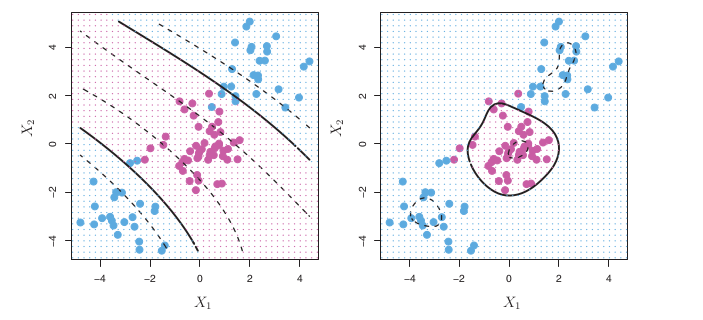
\includegraphics[width=\textwidth]{./chap/1chap/8sec/images/3polynomialRadialKernel.png}
	\end{center}
	\caption{Left: a SVM with a polynomial kernel of degree 3 is
	applied to non-linear data.\\
	Right: a SVM  with a radial kernel is applied.}
	\label{fig:8.3polynomialRadialKernel}
\end{figure}

\subparagraph{Python Code}
\begin{python}
import pandas as pd
import sklearn
from sklearn import tree
from sklearn import svm

y, X = df.iloc[:, 0], df.iloc[:, 1:]
clf = svm.SVC(
   C = 1.0, # Regularization parameter
   kernel = 'linear', # {'linear', 'poly', 'rbf'}
)
clf.fit(X, y)

\end{python}
